\section{Practical exercice: Polynomial evaluation}

Polynomial evaluation is a common source of computational error. Polynomials are frequently used for function interpolation in libraries or user codes. As we will see, different evaluations of the same polynomial do not have the same behavior in terms of performance or numerical accuracy.

This tutorial is uses the following Tchebychev polynomial from ~\cite[pp.52-54]{parker1997monte}:

$$T(x)=\sum_{i=0}^{10}{a_i \times x^{2i}}$$
With:
$a_i \in [
  1,
  \matminus 200,
  6600,
  \matminus 84480,
  549120,
  \matminus 2050048,
  4659200,
  \matminus 6553600,
  5570560,
  \matminus 2621440,
  524288
]$

We are interested in evaluating  $T$ near $1$.
This example is discussed with details in~\cite[pp.52-54]{parker1997monte}.

\subsection{Expanded form evaluation}

\subsubsection{First steps with Verificarlo}

In this first approach, we will evaluate the polynomial in its expanded form as given in the previous section. We first evaluate it in single precision. In this part of the tutorial we will work inside the \texttt{tchebychev/} folder.

\begin{question}
  \begin{enumerate}[(a)]
  \item Open the {\tt tchebychev.c} file and observe the function {\tt REAL expanded(REAL x)}.

  \item Compile {\tt tchebychev.c} with {\tt verificarlo} using the following command:
\begin{verbatim}
verificarlo -D FLOAT tchebychev.c -o tchebychev
\end{verbatim}
  \item Run the program.
  \end{enumerate}
\end{question}

When running the program it complains that at least one backend should be
selected with the \texttt{VFC\_BACKENDS} environment variable.
To run the program with standard IEEE-754 arithmetic one can use the simple
IEEE backend (\texttt{libinterflop\_ieee.so}). The backend has a \texttt{--debug}
option that shows the floating-point operations that have been instrumented.

\begin{question}
Run the program using the IEEE backend,
\begin{verbatim}
VFC_BACKENDS="libinterflop_ieee.so --debug" ./tchebychev 0.99 EXPANDED
\end{verbatim}
\end{question}

To evaluate the numerical error we will use the Monte Carlo arithmetic backend
(\texttt{libinterflop\_mca.so}.  Because we are using IEEE-754 floats, to
simulate round-off errors we should work at a 24 bits precision.

\begin{question}
  \begin{enumerate}[(a)]
  \item Run the program using the Monte Carlo Arithmetic backend at 24 bits precision,
\begin{verbatim}
VFC_BACKENDS="libinterflop_mca.so --precision=24" ./tchebychev 0.99 EXPANDED
\end{verbatim}
  \item Execute the program multiple times. What can you observe?
  \end{enumerate}
\end{question}

Monte Carlo arithmetic backend supports different modes,
\begin{itemize}

  \item \texttt{-{}-mode=rr} is the \emph{random round} mode that adds noise on the
    result of an operation only when the operation is not exactly representable
    at the given precision. This mode is useful to simulate the effect of
    round-off errors.

  \item \texttt{-{}-mode=pb} is the \emph{precision bound} mode that adds noise on
  the operands before performing the operation. It is useful to simulate the
    effect of cancellations errors.

  \item \texttt{-{}-mode=mca} is the default mode that combines \texttt{rr} and
  \texttt{pb} modes.

\end{itemize}

\begin{question}
  \begin{enumerate}[(a)]
  \item Now recompile with verificarlo the program in double precision using the command
    {\tt verificarlo -D DOUBLE tchebychev.c -o tchebychev} \\
  \item Execute the program with arguments \texttt{0.99 EXPANDED} with the Monte Carlo arithmetic backend. Try different precisions such as 53, 24, 10. Try also to use different modes (rr, pb, mca).
  \end{enumerate}
\end{question}

\subsubsection{Numerical quality analysis}

In this section, we propose you to analyze the numerical quality of the results
computed by the expanded evaluation of the polynomial. To simplify this task,
you can use the script~\texttt{run.sh} which automates the required verificarlo
runs. Visualization is done using the \texttt{plot.py} script.


\begin{question}
  \begin{enumerate}[(a)]
 \item Open {\tt run.sh} and understand how it works.
  \item Modify {\tt run.sh} to evaluate the polynomial in the interval $[0.5,1]$ by $0.001$ step.
  \item Open {\tt plot.py} and understand how it works, and what is the plotted data.
  \end{enumerate}
\end{question}

Figure~\ref{fig:expanded:double:24} is generated with the \texttt{plot.py} script.

The lowest part are the $T(x)$ samples and their average in dotted line. The 20 Monte Carlo samples $T(x)$ are plotted for each $x$ value (sometime overlapping on the graphic)
The central part is the empirical standard deviation $\hat\sigma$ for each value of $x$.
The upper part of the figure represents the number $s$ of significant digits of each output: $s=-\log_{10}\left|\dfrac{\hat\sigma}{\hat\mu}\right|$ with $\hat\sigma$ the sample empirical standard deviation  $\hat\mu$ their average.

\begin{question}
\begin{enumerate}[(a)]
\item To execute the {\tt EXPANDED} version with {\tt DOUBLE} and a virtual precision of 24 bits, execute the command: {\tt ./run.sh EXPANDED
      DOUBLE 24 mca}. \newline This command's output is given in figure~\ref{fig:expanded:double:24}.
  \item With a virtual precision of 53, execute the command: {\tt ./run.sh EXPANDED DOUBLE 53 mca} \newline
  This command's output is given in figure~\ref{fig:expanded:double:53}.
  \end{enumerate}
\end{question}

\begin{figure}[h]
\center 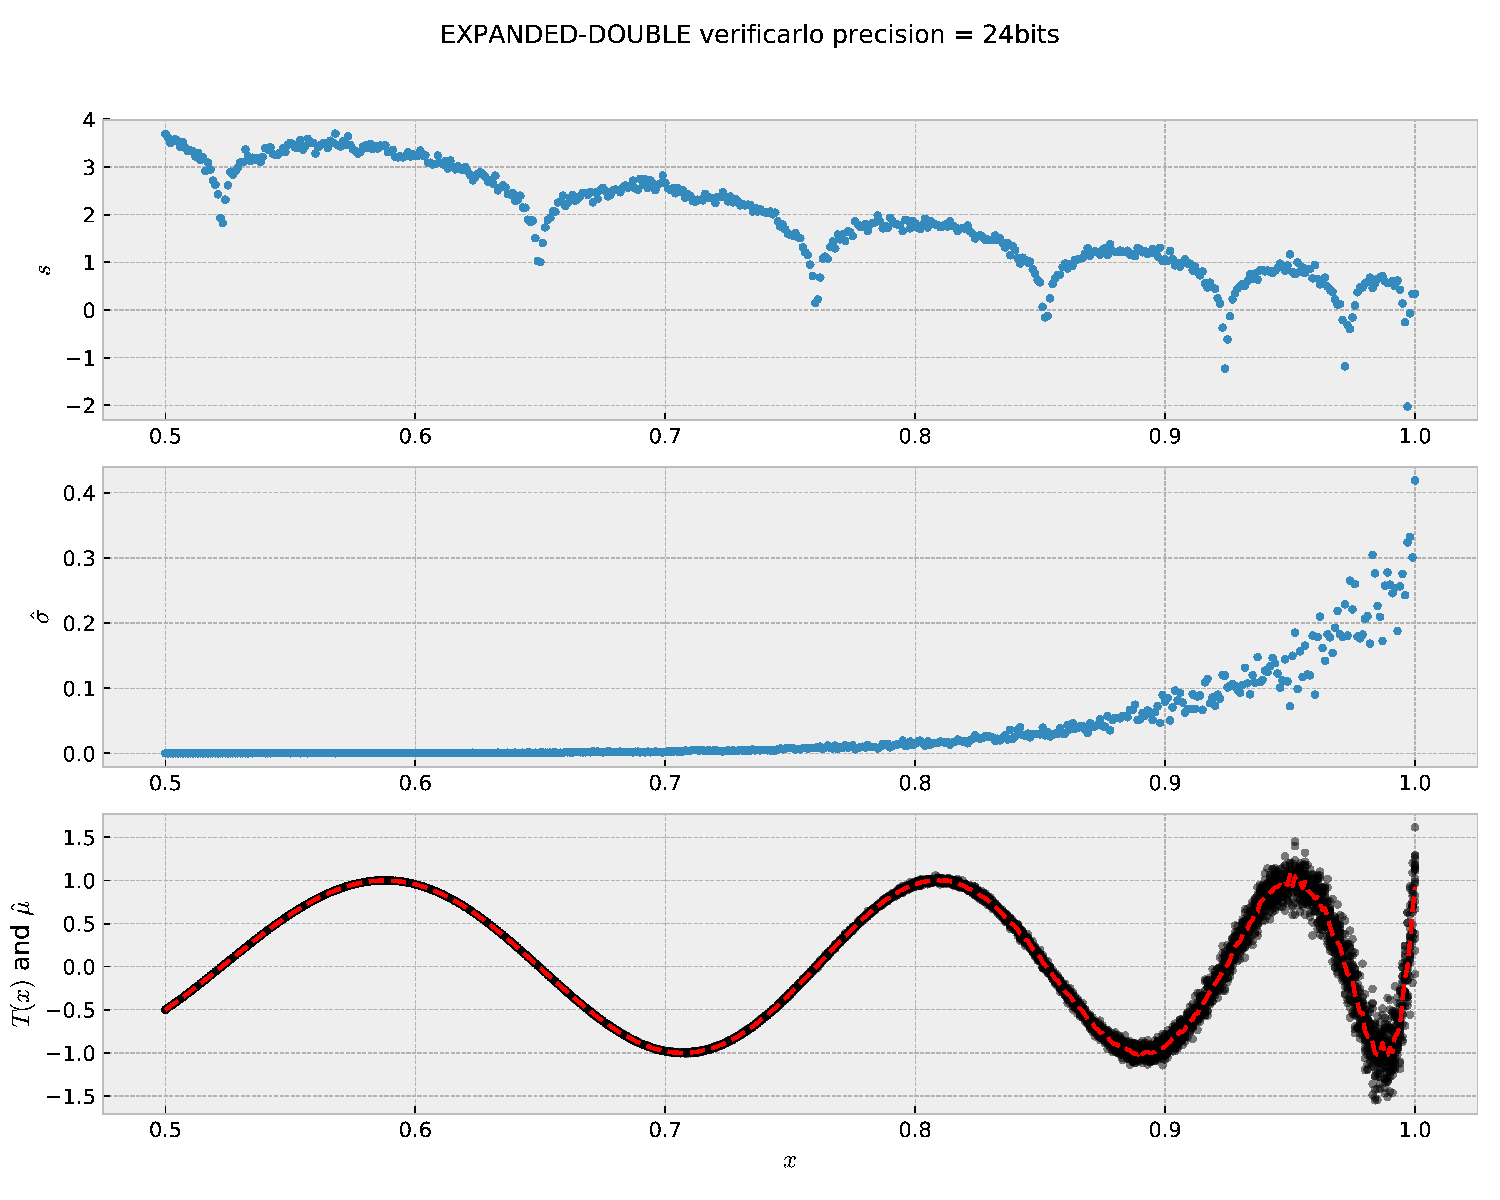
\includegraphics[width=.8\textwidth]{EXPANDED-DOUBLE-24.pdf}
  \caption{Evaluation of T(x) in its expanded form, compiled in double precision, with a virtual precision of 24}
  \label{fig:expanded:double:24}
\end{figure}
\begin{figure}[h]
\center 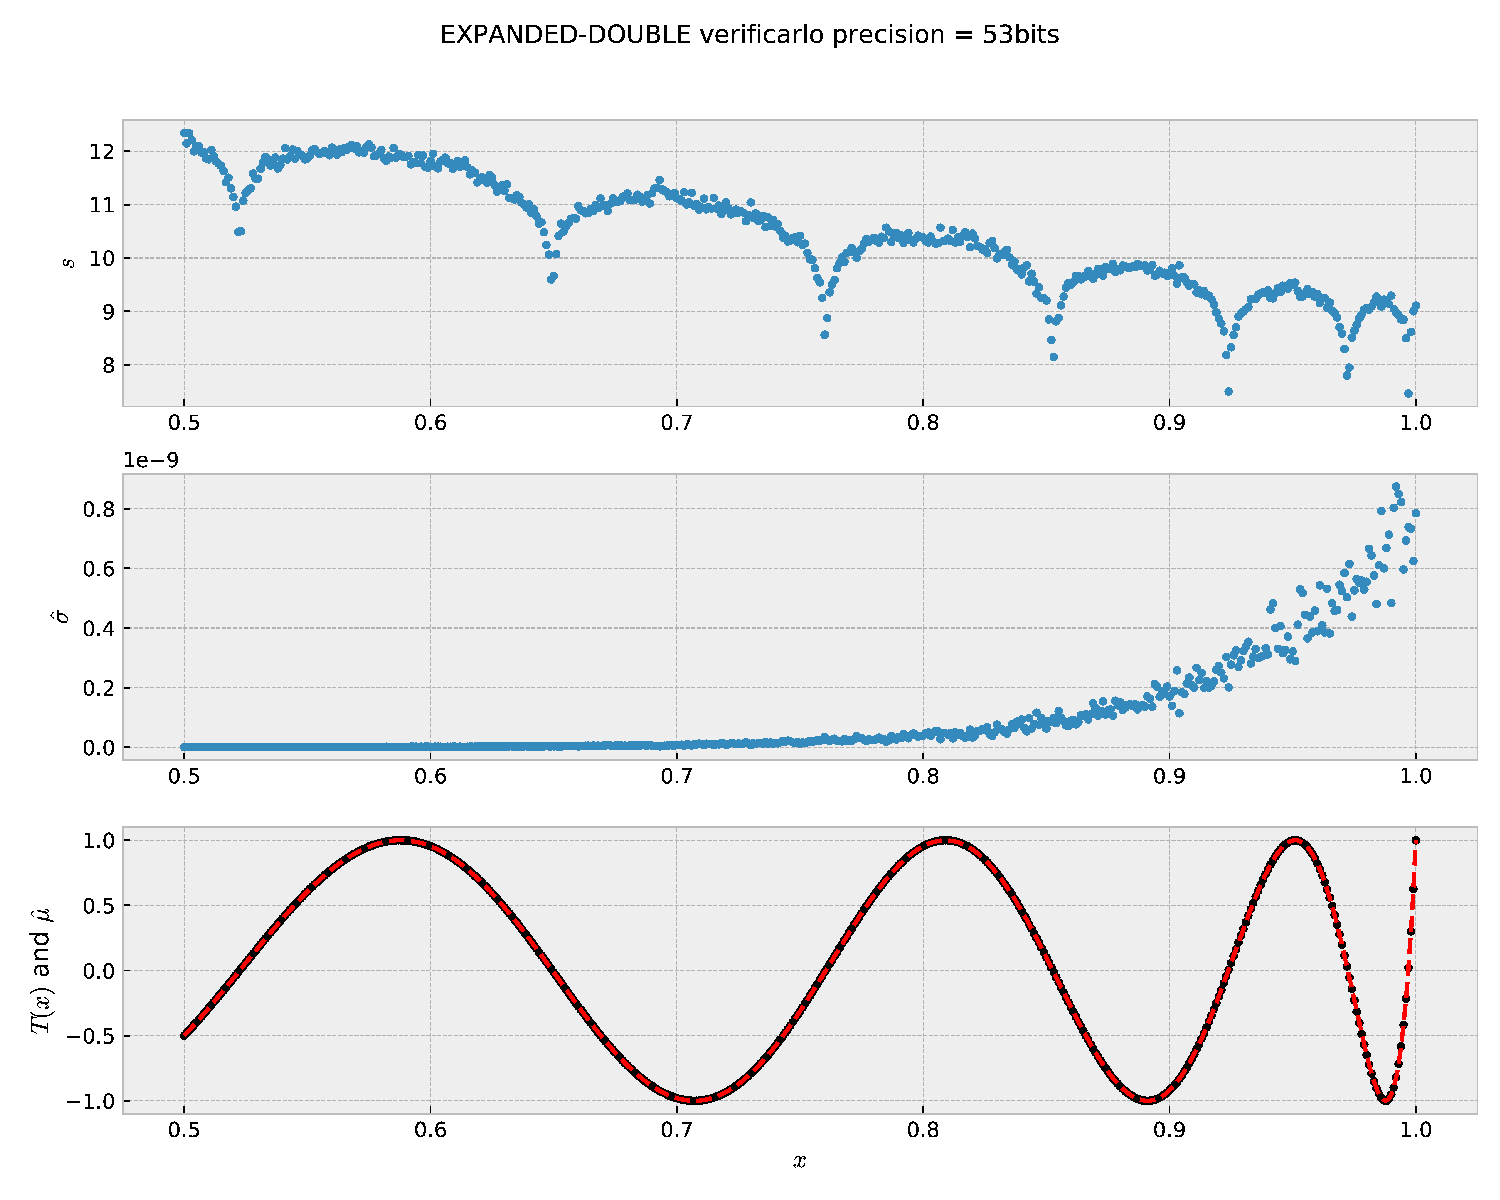
\includegraphics[width=.8\textwidth]{EXPANDED-DOUBLE-53.pdf}
  \caption{Evaluation of T(x) in its expanded form, compiled in double precision, with a virtual precision of 53}
  \label{fig:expanded:double:53}
\end{figure}

Close to 1, the polynomial evaluation is subject to {\it cancellations} which
rapidly decrease the result precision. The double precision on the contrary
seems satisfactory.  However using double precision forces the programmer to
use a larger and more costly data type and the cancellations still happen when
getting closer to 1.  Nevertheless if the user is already using double
precision number, and if the precision is still not satisfactory, how to solve
the issue? Or what if our hardware only implements single precision?

\FloatBarrier

\subsection{Evaluation using Horner scheme}

Multiple ways to evaluate polynomials exist, using associativity, commutativity and factorization. More often they are explored for the sake of performance, but they also greatly influence the precision of the evaluation. One of them reputed to combine both performance and good numerical behavior is the Horner scheme which for our polynomial correspond to the following form:

\[
	T(x) = (\dots((a_n\times x^2 + a_{n-1})\times x^2 + a_{n-2})\dots) \times x^2
    + a_0
\]

$$T(x) = (((((((((524288*x^2-2621440)*x^2+5570560)*x^2-6553600)*$$
$$x^2+4659200)*x^2-2050048)*x^2+549120)*x^2-84480)*$$
$$x^2+6600)*x^2-200)*x^2+1$$

\begin{question}
  \begin{enumerate}[(a)]
  \item Open the file {\tt tchebychev.c} and have a look to the function {\tt REAL horner(REAL x)}
\item While keeping previous execution parameters, execute the command {\tt ./run.sh HORNER DOUBLE 53 mca}.  \newline The output of this command is given in figure~\ref{fig:horner:double:53}.
  \end{enumerate}
\end{question}

\begin{question}
\item Execute the command {\tt ./run.sh HORNER DOUBLE 24 mca}  \newline
The output of this command is given in figure~\ref{fig:horner:double:24}.
\end{question}

As shown in this experiment, the Horner scheme does not improve much the result
precision ($\simeq$ 1 additional significant bit). However, it minimizes the
number of operations and allows to use the FMA ({\it Fused Multiply Add}). For
a polynomial of degree $n$, it produces $n-1$ FMA. Moreover, when doing
multiple independent evaluations it can be vectorized.

\begin{figure}[htb]
\center 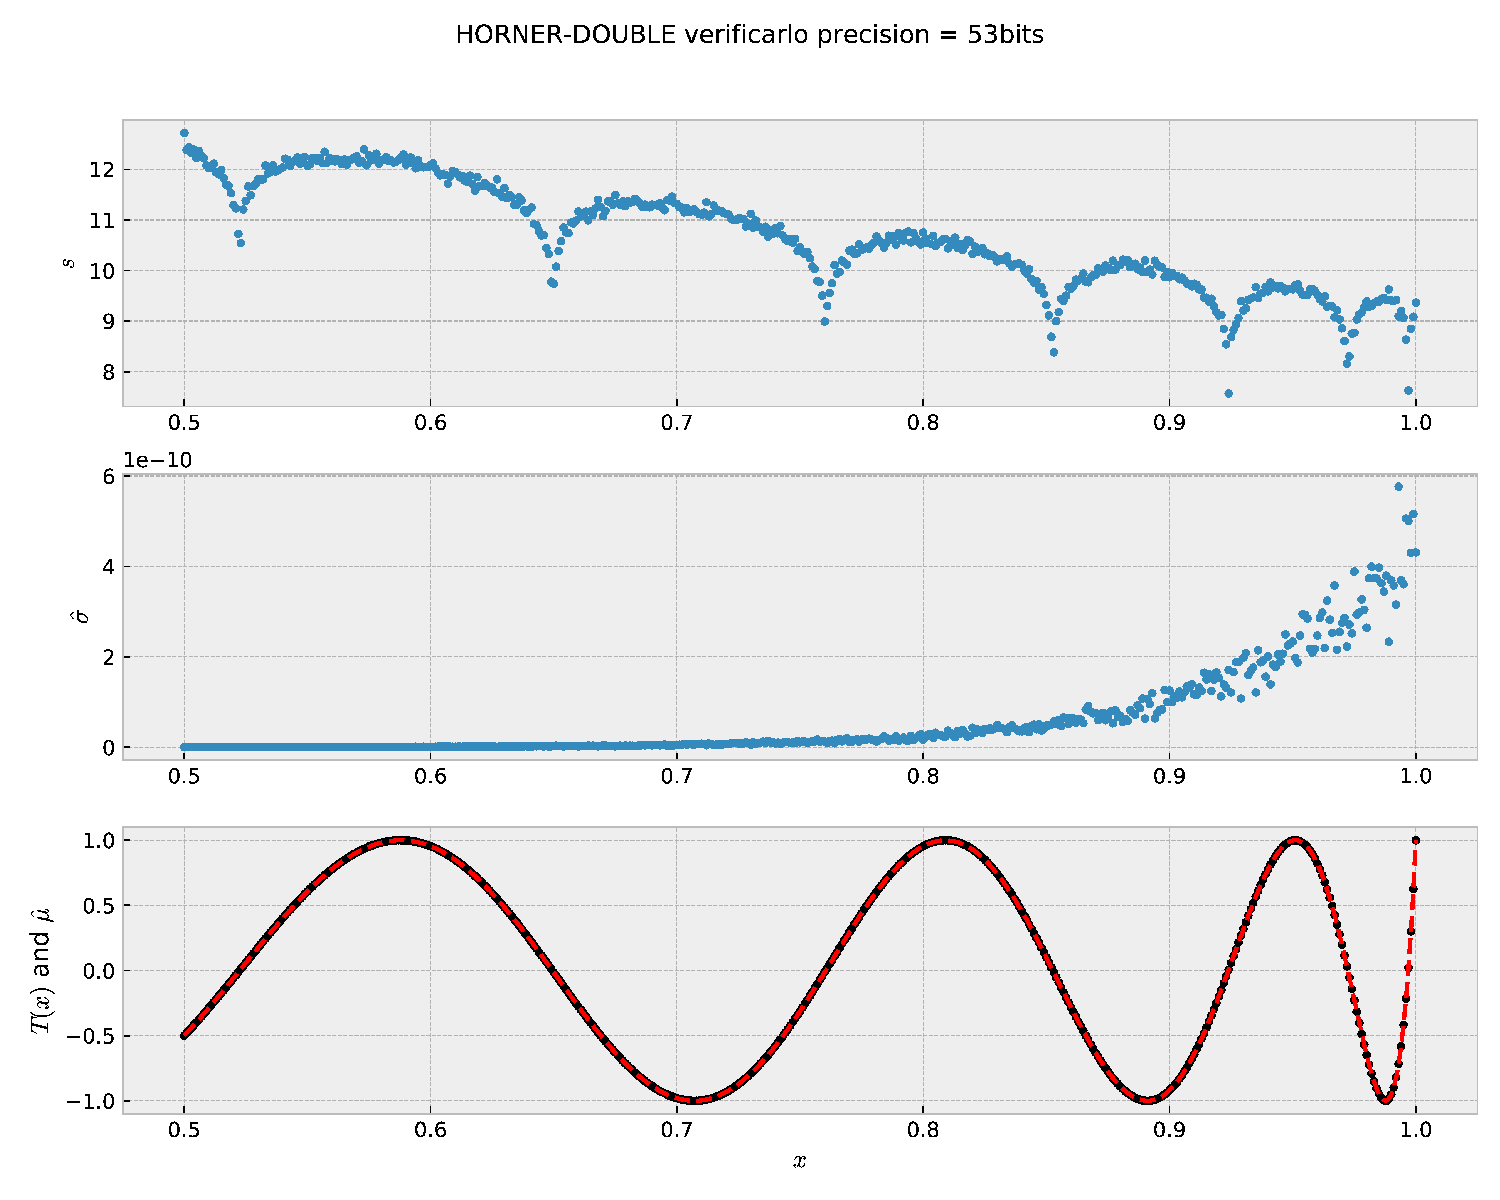
\includegraphics[width=.8\textwidth]{HORNER-DOUBLE-53.pdf}
  \caption{Evaluation of T(x) using Horner scheme, compiled in double precision, with a virtual precision of 53}
  \label{fig:horner:double:53}
\end{figure}
\begin{figure}[htb]
\center 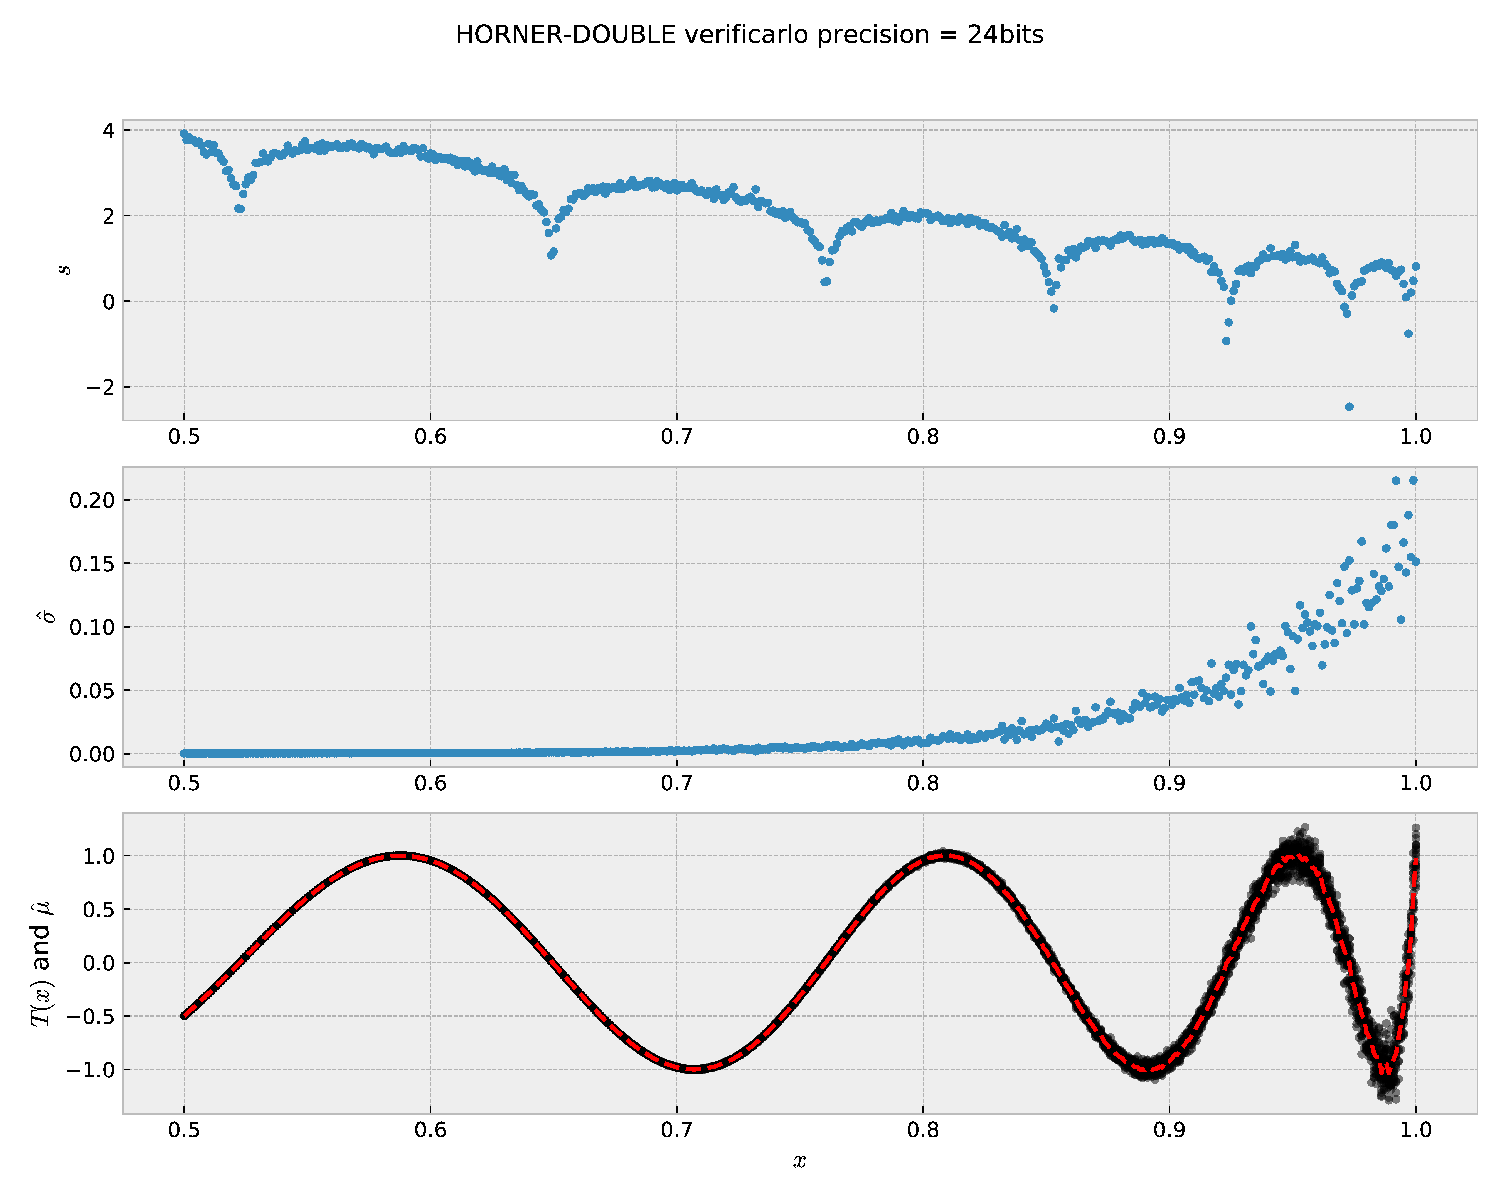
\includegraphics[width=.8\textwidth]{HORNER-DOUBLE-24.pdf}
  \caption{Evaluation of T(x) using Horner scheme, compiled in double precision, with a virtual precision of 24}
  \label{fig:horner:double:24}
\end{figure}
